\begin{figure}
	\center
	\includegraphics[trim={0 10 0 0}, clip, width=\linewidth]{vect/dataset_ex}
	\caption{\label{fig:dataset} \textbf{Examples of test images :} we compare our new localization method on four challenging localization sequences. The number under the query set name indicates the amount of images to localize according to the 1688 reference images.}
\end{figure}

\section{Experiments}
\label{sec:experiments}

\subsection{Dataset}
\label{subsec:dataset}
	We have tested our new method on the \textit{Oxford Robotcar} public dataset~\cite{Maddern2016}. This is a common dataset used for image based localization~\cite{Sattler2018} and loop closure algorithm involving neural networks training~\cite{Porav2018}.
		
\vspace{4pt}\noindent\textbf{Training data.}
	We use dataset temporal redundancy to build our images triplets to train our CNN. We build 400 triplets using three runs acquired at dates: \texttt{2015-05-19, 2015-08-28} and \texttt{2015-11-10}. We selected a different area of city Oxford than the one used for training our networks for validation.
	Depth modality from \textit{Oxford Robotcar} dataset is extracted from the lidar point cloud. When re-projected in the image frame coordinate, it produces a sparse depth map. Since deep convolutional neural networks require dense data as input, we pre-process these sparse modality maps with inpainting algorithm from~\cite{Bevilacqua2017} in order to make them dense.

\vspace{4pt}\noindent\textbf{Testing data.} We propose four testing scenarios on the same spatial area, separate from both training and validation area. Reference dataset is composed of 1688 images taken every 5 meters along a path of 2 km when the weather was overcast. The four query sets are:
	\paragraph{Sunny/Overcast} queries have been acquired during a sunny day.
	\paragraph{Long-term} queries have been acquired 7 months after the reference images under similar weather conditions.
	\paragraph{Winter/Summer} queries have been acquired during a snowy day.
	\paragraph{Night/Day} queries have been acquired at night, resulting in radical visual changes compare to the reference images.

Query examples are presented in figure~\ref{fig:dataset}.
	
\vspace{4pt}\noindent\textbf{Evaluation metric.} For a given query, reference images are ranked according to the cosine similarity score computed over their descriptors. To evaluate the localization performances, we consider two evaluation metrics:
	\setcounter{paragraph}{0}
	\paragraph{Recall @N} we plot the percentage of well localized queries regarding the number $N$ of returned candidates. A query is considered well localized if one of the top $N$ retrieved images lies inside the $25m$ radius of the ground truth query position.
	\paragraph{Top-1 recall @D} We compute the distance between the top ranked returned database image position and the query ground truth position, and report the percentage of queries located under a threshold D (from 15 to 50 meters), like in~\cite{Zamir2014}. This metric qualifies the accuracy of the localization system.

\subsection{Implementation details}
\label{subsec:implementation}

For our methods implementation we use Pytorch as deep learning framework, ADAM stochastic gradient descent algorithm for the CNN training with learning rate set to 1e-4, weight decay to 1e-3 and $\lambda$ in triplet loss equations~\ref{eq:triplet_loss},~\ref{eq:depth_triplet_loss},~\ref{eq:cat_triplet_loss} equal to 0.1. We use batch size between 10 and 25 triplets depending of the size of the system to train, convergence is occurring rapidly and take around 30 to 50 epochs. We perform both positive and negative hard minning, as in~\cite{Radenovic2017}. Images and depth maps are resized to 224x224 pixels before training and testing.

\vspace{4pt}\noindent\textbf{Encoder architectures.} We test Alexnet (A) and Resnet18 (R) network architectures for features map extraction. We drop the last pooling layer and the fully connected part for both architectures. The size of the final features block is 256*13*13 for Alexnet and 512*7*7 for Resnet. Initial weights are the ones obtained by training the whole network on ImageNet dataset.

We always use Alexnet encoder to extract features from raw depth map, reconstructed depth map, or hallucinated depth map. Indeed the quality of our depth map are very low, we have found that using deeper network do not significantly improves localization results.

\vspace{4pt}\noindent\textbf{Descriptor architectures.} We test the two state of the art image descriptors MAC~\cite{Radenovic2017} and NetVLAD~\cite{Arandjelovic2017}. MAC is a simple global pooling method that takes the maximum of each feature map from the encoder output. MAC combined with Alexnet encoder produces a 256 dimensional descriptor, whereas combined with Resnet architecture it produces a 512 dimensional descriptor.

NetVLAD is a trainable pooling layer that mimics VLAD aggregation method. For all the experiments, we set the number of clusters to 64, resulting in a 16~384 dimensional descriptor if it is used with Alexnet features and a 32~768 dimensional if Resnet features are used instead. The dimension of the final descriptor can be drastically reduced with PCA-whitening post-processing.

Finally, both MAC and NetVLAD descriptors are $L_{2}$ normalized.

\vspace{4pt}\noindent\textbf{Decoder architecture.} The decoder used in our proposal (see figure~\ref{fig:our_method}) is based on Unet architecture and inspired by network generator from~\cite{Isola2017}. Dimension up-sampling is performed through inverse-convolutions layers. Decoder weights are initialized randomly.

\subsection{Results}
\label{subsec:results}

\begin{figure}
	\center
	\begin{minipage}{0.49\linewidth}
		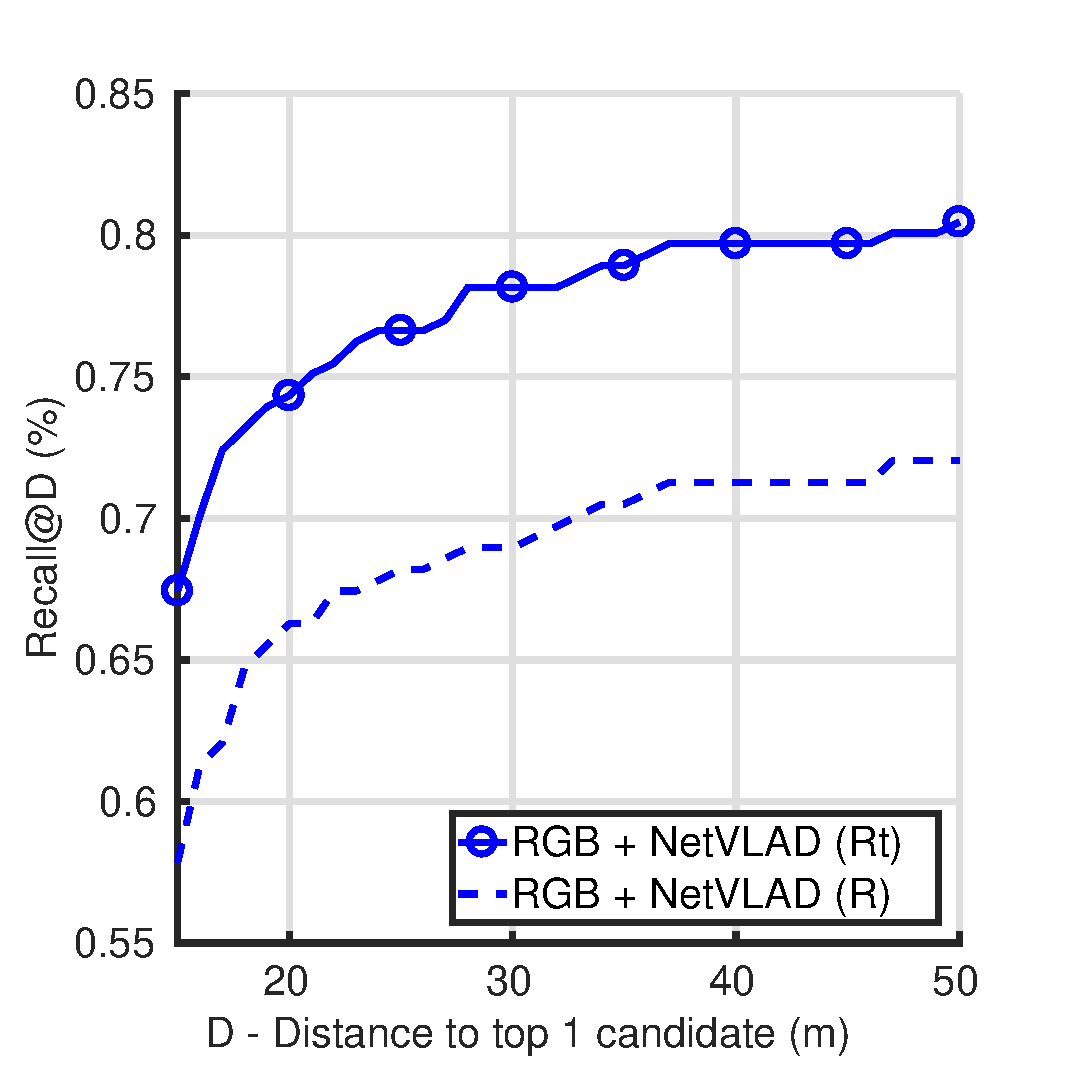
\includegraphics[width=\linewidth]{plot/fig/rgb_r_trunc_distance}	
	\end{minipage}
	\begin{minipage}{0.49\linewidth}
		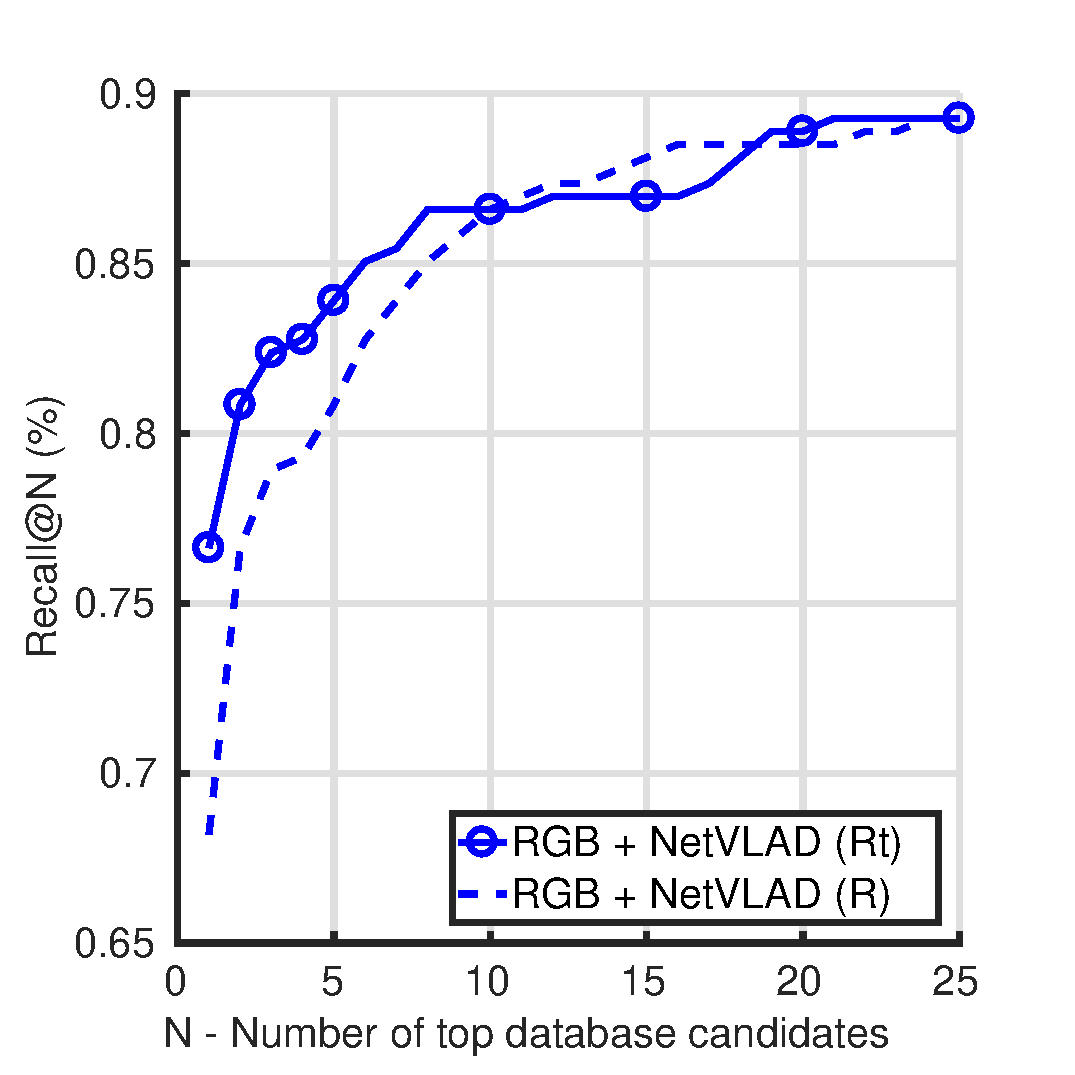
\includegraphics[width=\linewidth]{plot/fig/rgb_r_trunc_recall}	
	\end{minipage}
	\caption{\label{fig:trunc_resnet} \textbf{Resnet18 (R) versus truncated Resnet18 (Rt) in combination with NetVLAD pooling:} we show the importance of spatial resolution of the deep feature maps of the encoder used with NetVLAD layer. The truncated version of Resnet18, more than two time lighter the complete one, achieve much better localization results.}
\end{figure}

\begin{figure*}
	\center
	\begin{minipage}{0.14\linewidth}
		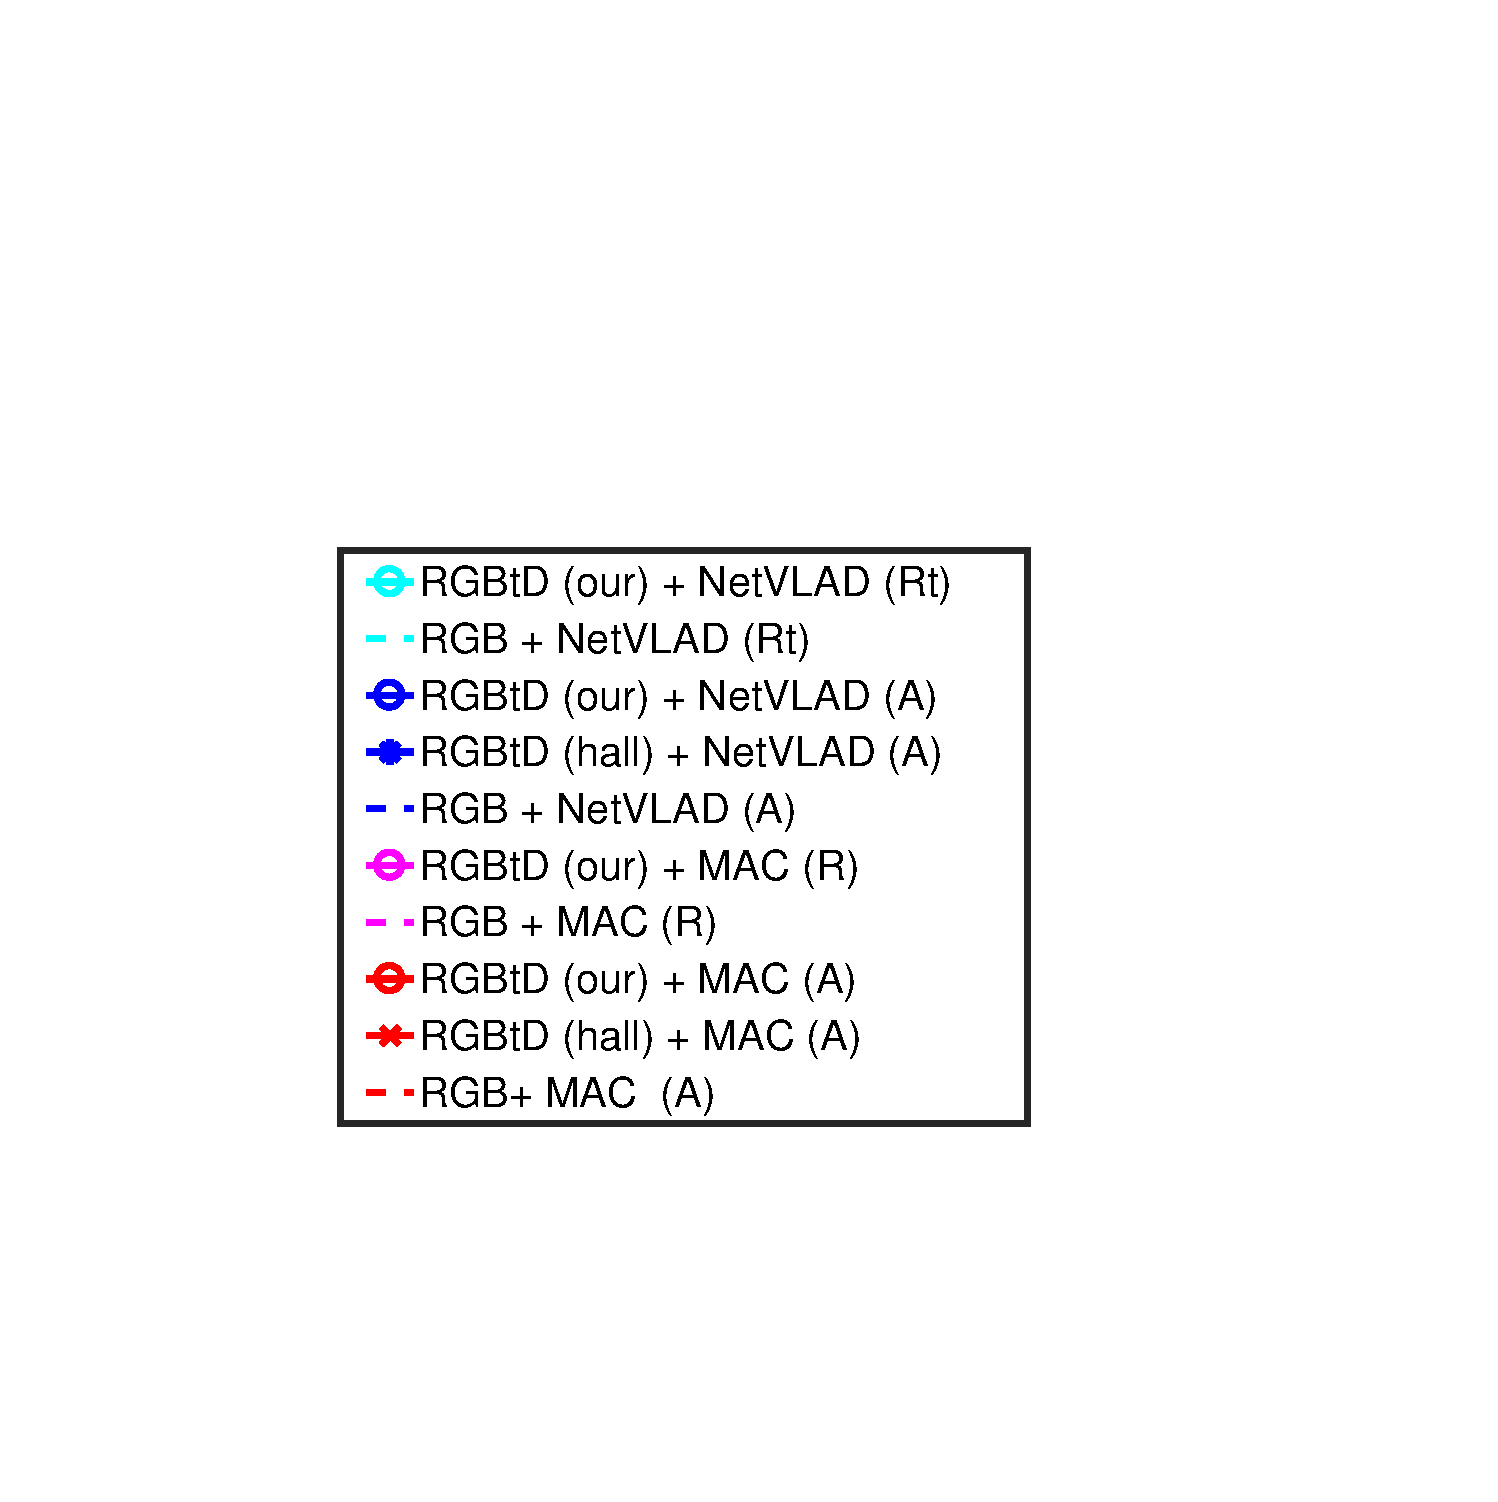
\includegraphics[trim={90 140 95 100},clip,width=\linewidth]{plot/fig/legend}	
	\end{minipage}
	\begin{minipage}{0.85\linewidth}
	
	\begin{minipage}{0.49\linewidth}		
		\center
		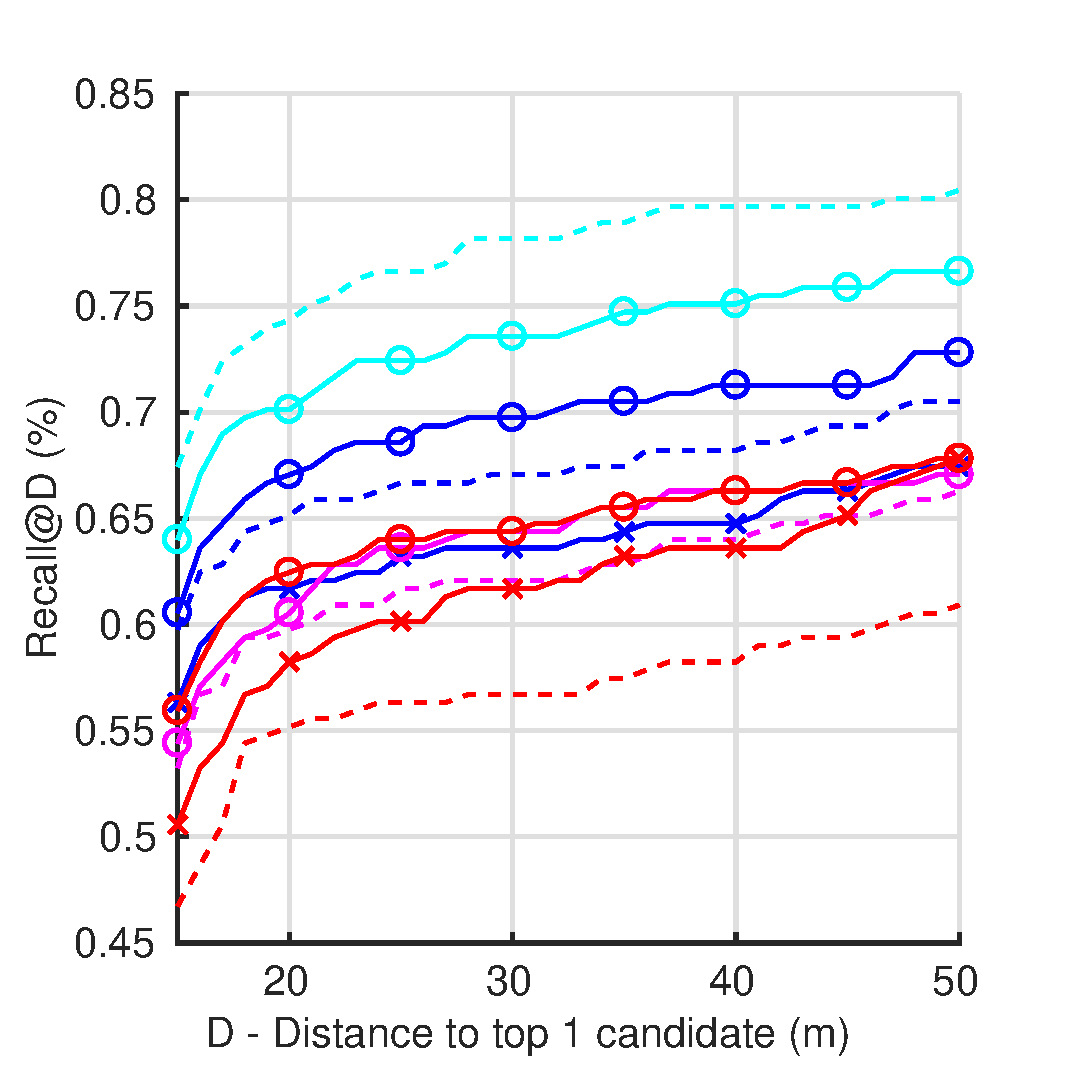
\includegraphics[width=0.49\linewidth]{plot/fig/sun_distance}	
		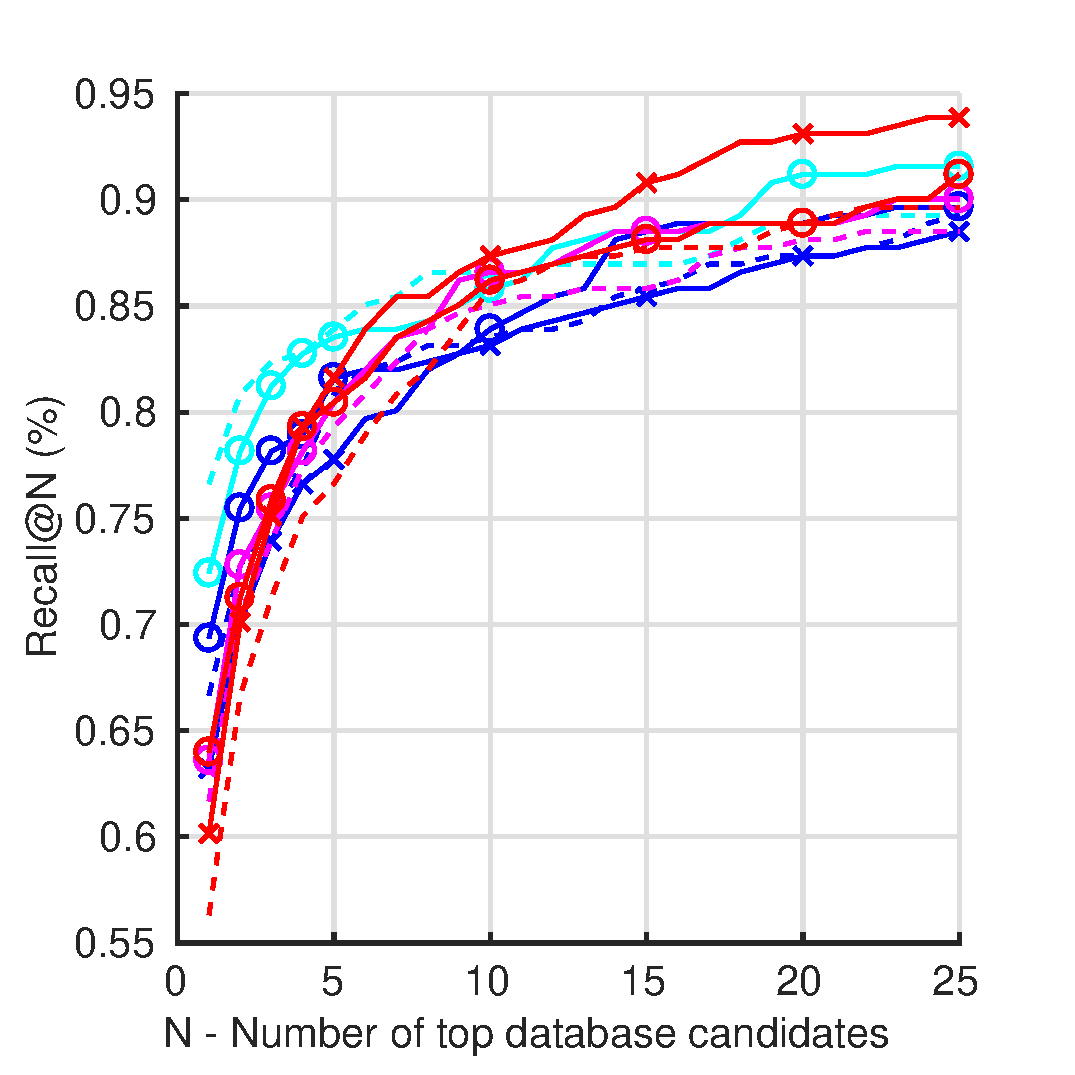
\includegraphics[width=0.49\linewidth]{plot/fig/sun_recall}
		
		{\scriptsize a) Sunny/Overcast}
	\end{minipage}
	\begin{minipage}{0.49\linewidth}
		\center
		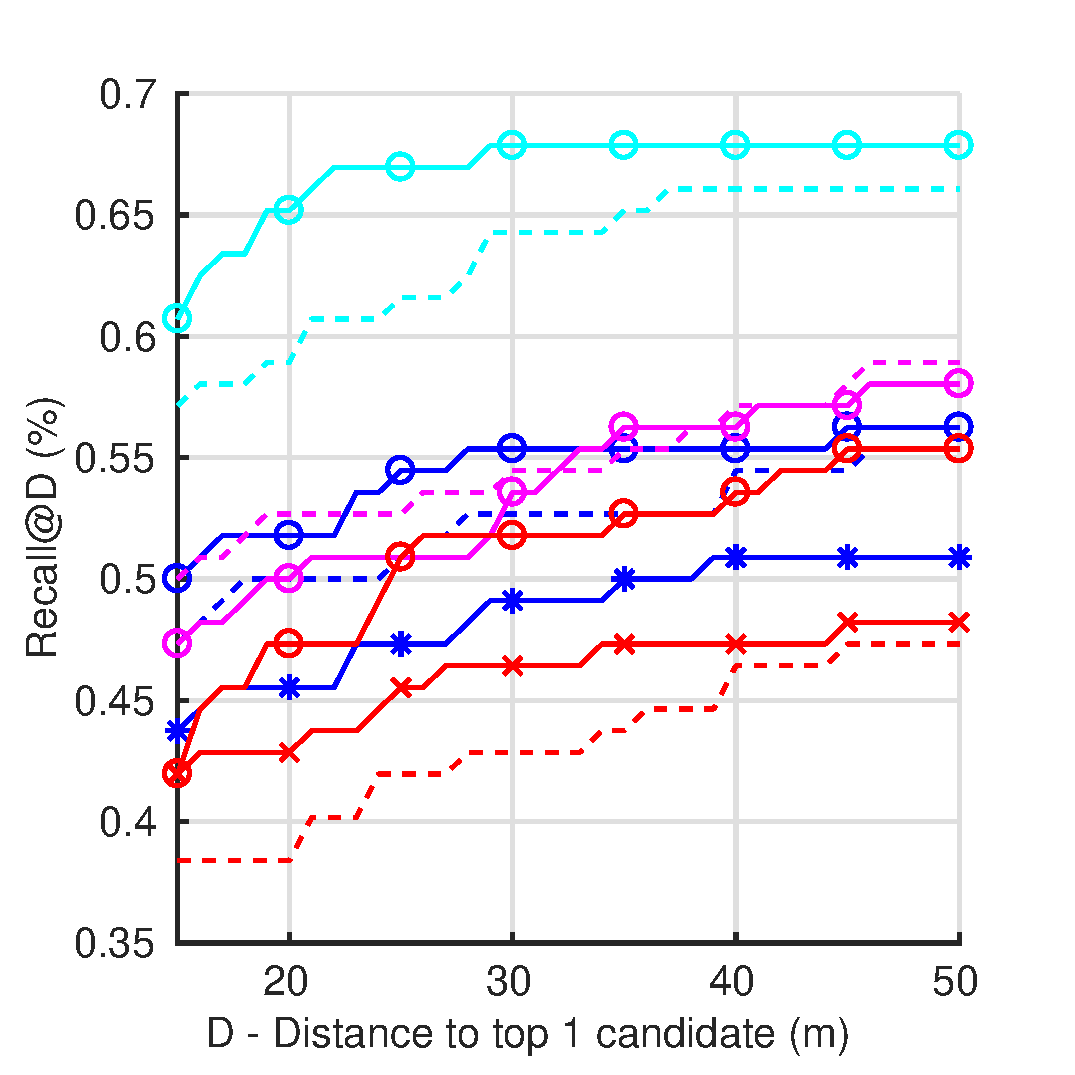
\includegraphics[width=0.49\linewidth]{plot/fig/snow_distance}	
		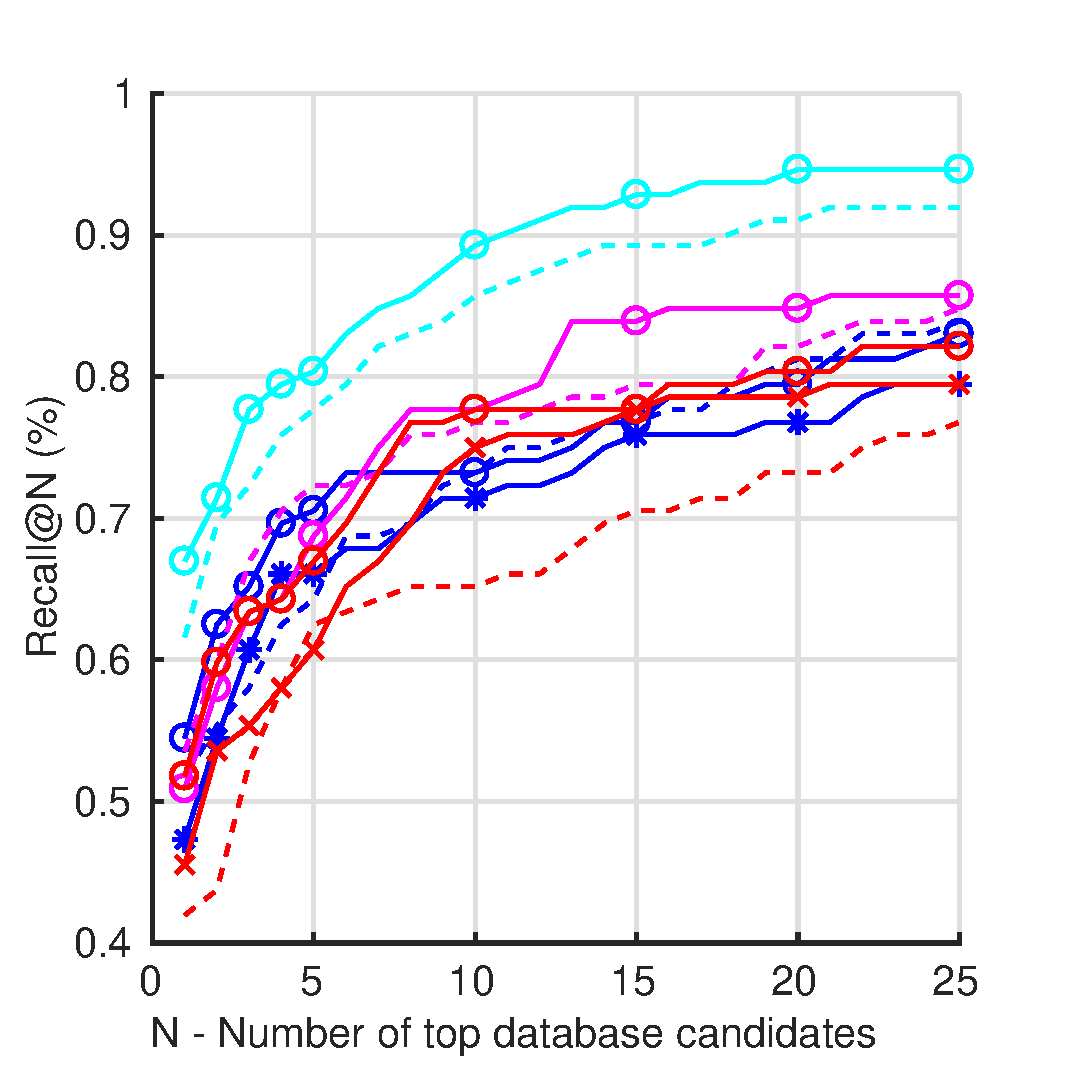
\includegraphics[width=0.49\linewidth]{plot/fig/snow_recall}
		
		{\scriptsize b) Winter/Summer}
	\end{minipage}
	
	\begin{minipage}{0.49\linewidth}
		\center
		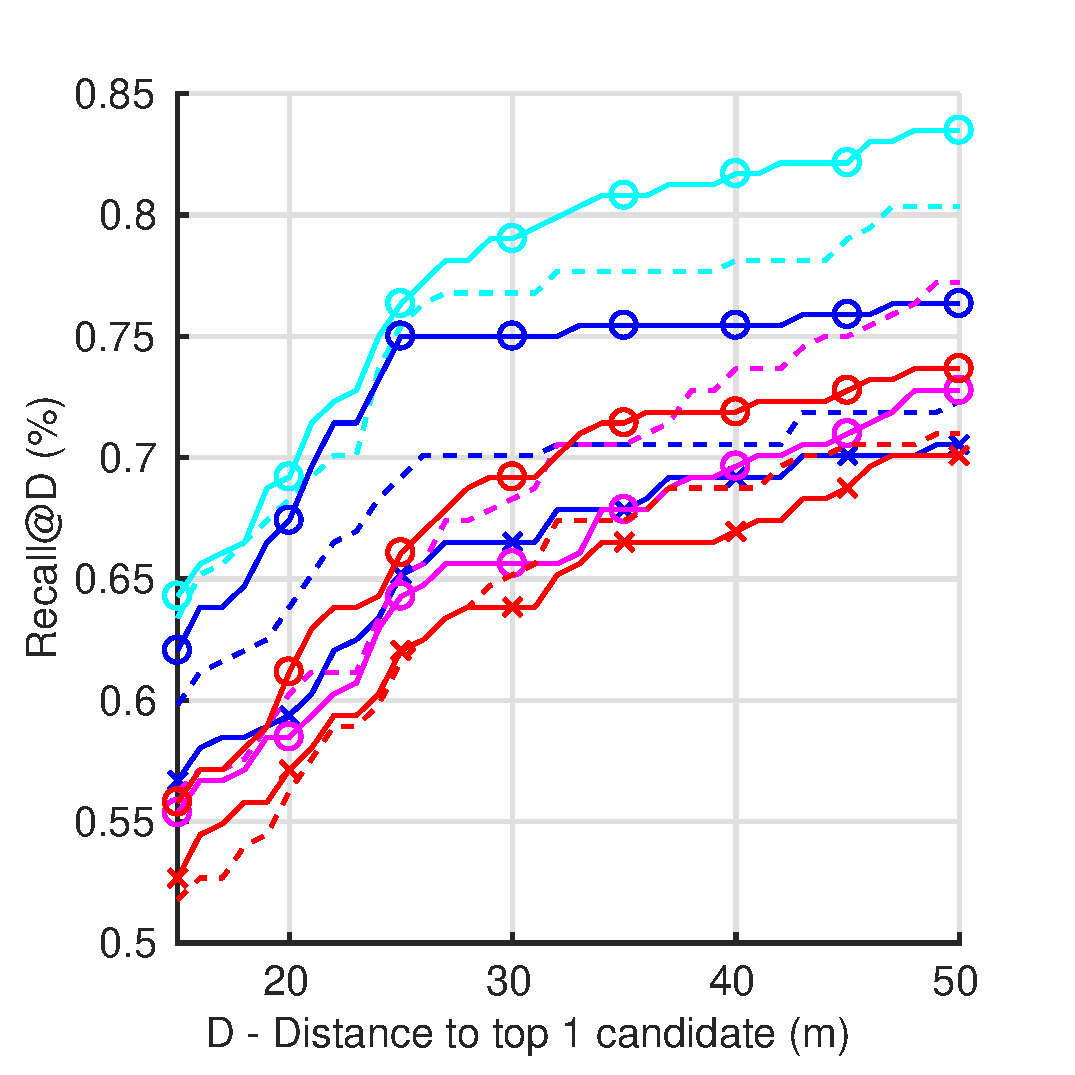
\includegraphics[width=0.49\linewidth]{plot/fig/lt_distance}	
		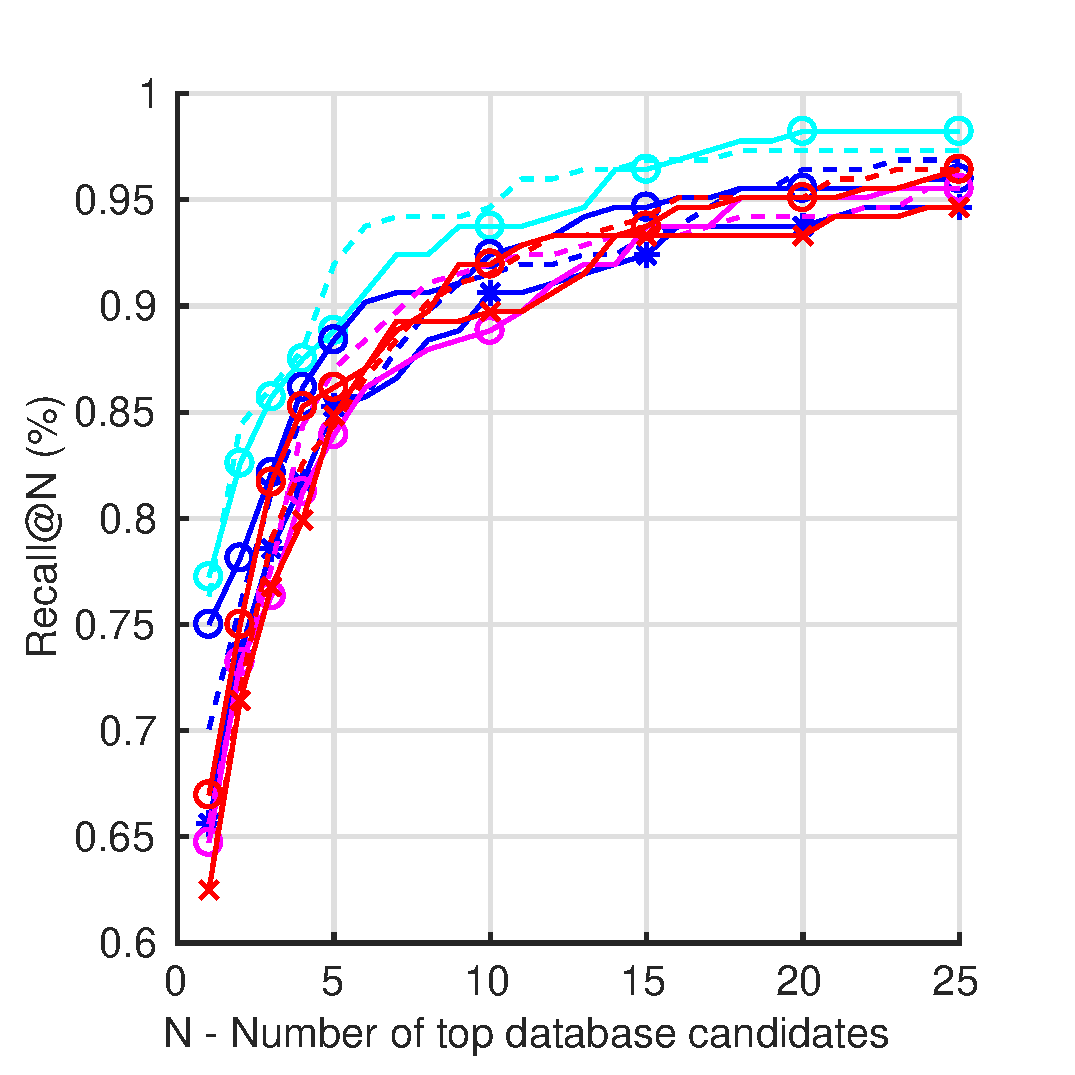
\includegraphics[width=0.49\linewidth]{plot/fig/lt_recall}

		{\scriptsize c) Long-term}		
	\end{minipage}
	\begin{minipage}{0.49\linewidth}
		\center	
		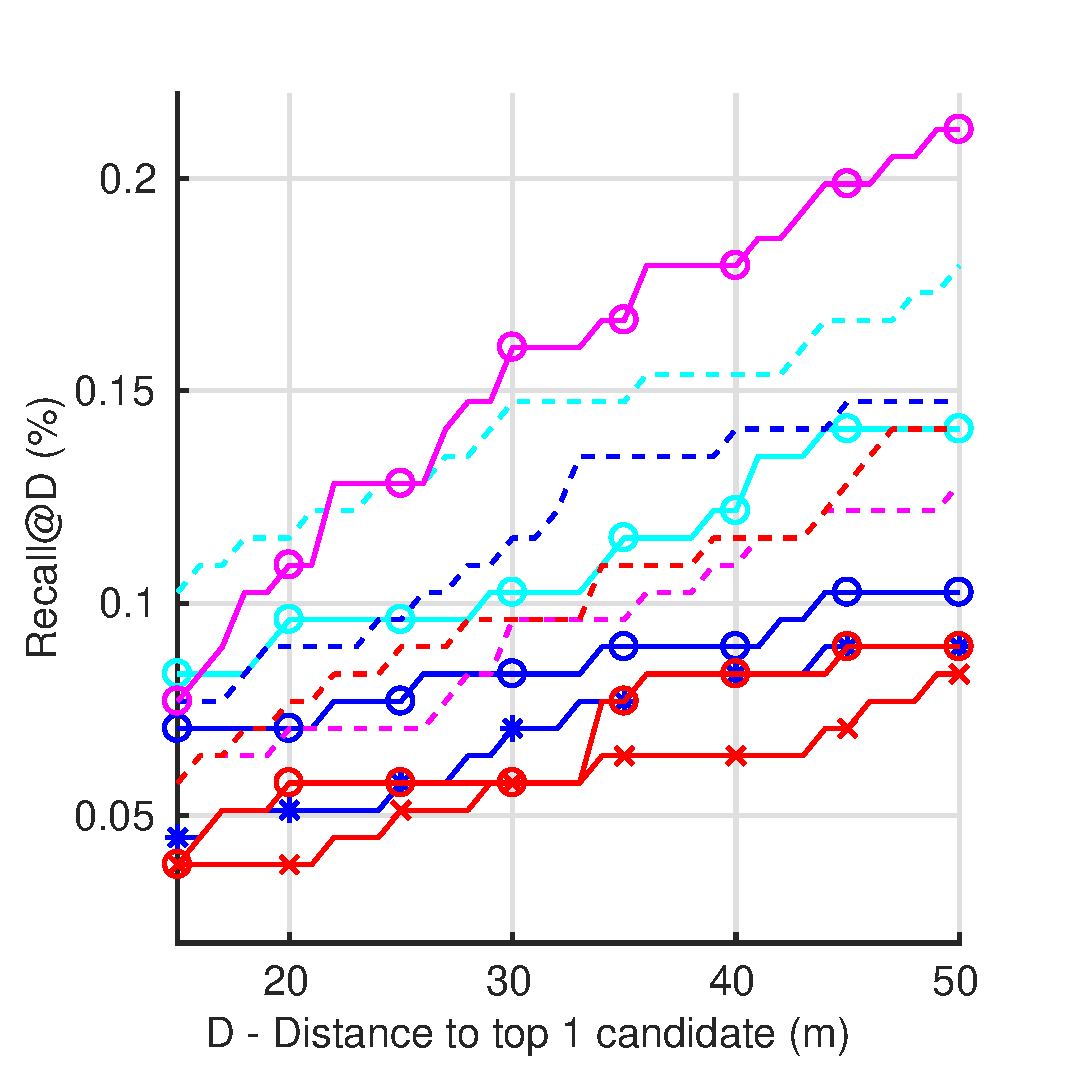
\includegraphics[width=0.49\linewidth]{plot/fig/night_distance}	
		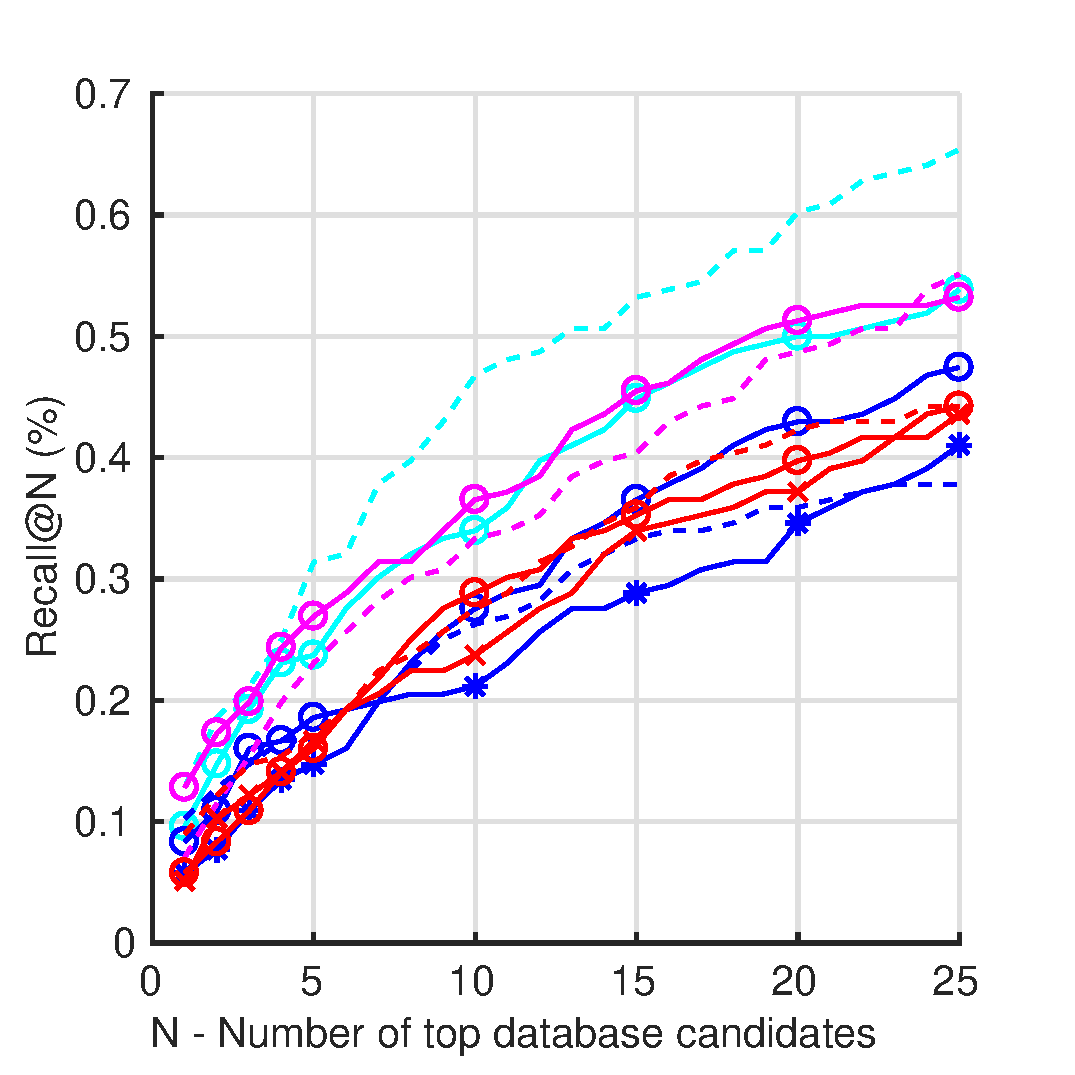
\includegraphics[width=0.49\linewidth]{plot/fig/night_recall}
	
		{\scriptsize d) Night/Day}
	\end{minipage}
	
	\end{minipage}

	\caption{\label{fig:results} \textbf{Comparison of our method versus hallucination network and networks trained with only images}: our method (-o-) is superior in almost every scenario compare to hallucination network (-x-). It also beats by a significant margin networks trained with only images (\texttt{--}). NetVLAD descriptors (\textcolor{blue}{blue} and \textcolor{cyan}{cyan} curves) are superior to MAC (\textcolor{red}{red} and \textcolor{magenta}{magenta} curves), specially in term of accuracy (Recall@D curve). Night/day dataset remains the most challenging one. Best viewed in colors.}
\end{figure*}

\noindent\textbf{Baselines.} We compare our method with two state of the art baselines:
    \paragraph{RGB only (\textbf{RGB})} simple networks composed of encoder + descriptor trained with only images, without side depth maps information. We evaluate 4 variants of networks by combining Alexnet (A) or Resnet (R) encoder with MAC or NetVLAD descriptor pooling.
    \paragraph{RGB with Depth side information (\textbf{RGBtD})} networks that use pairs of aligned \{image/depth map\} during training step and images only at test time. We compare the proposed approach (ours) with our version of hallucination network~\cite{Hoffman2016} (hall). We follow training procedure of~\cite{Hoffman2016} to train the hallucination network, whereas our proposal is trained as explained in~\ref{subsec:training}. 

\vspace{4pt}\noindent\textbf{Truncated Resnet.} We found that NetVLAD descriptor combined with Resnet architecture, RGB + NetVLAD (R), do not perform well. NetVLAD can be view as a pooling method that acts on local deep features densely extracted from the input image. We argue that the spatial resolution of the features block obtained with Resnet encoder is too low compare to the other architecture (for instance 13*13 for Alexnet compare to 7*7 for Resnet for an 224*224 input image). We propose a truncated version of Resnet encoder (Rt), created by drooping the end of the network after the 13th convolutional layer. Thus we obtain a feature block with greater spatial resolution: 256*14*14 compare to 512*7*7. Recall results on the \textit{Sunny/Overcast} query set for both architectures are presented in figure~\ref{fig:trunc_resnet}. As the truncated version of Resnet encoder clearly dominated the full one, we use the truncated version for the following experiments.

\vspace{4pt}\noindent\textbf{Discussion.} Localization results on the four query sets are presented in figure~\ref{fig:results}.  When we use encoder architecture Alexnet combined with MAC descriptor, our system obtains a mean of +5\% on recall@1 score comparing to hallucination (on sun, long-term and winter query sets). The proposed method is also more accurate, obtaining a mean of +2.3\% on top-1 recall@15 and +3.7\% on top-1 recall@50 scores. These results demonstrate the superiority of our method compare to hallucination for the task of image localization. Both of the RGBtD approaches increase localization results compare to the RGB baseline (+7.3\% recall@1, +5.6\% top-1 recall@15, +5.9\% top-1 recall@50 for RGBtD (ours) versus RGB).

Results show that NetVLAD pooling is much more effective than MAC. However, we have not been able to obtain convincing results for hallucination network with Alexnet encoder combined with NetVLAD pooling: reported results show decreasing performances compare to RGB + NetVLAD (A) baseline. We do not investigate further on the hallucination method. Our proposal achieves superior localization scores with setting Alexnet encoder with NetVLAD descriptor compare to the RGB baseline: 62.85\%~/~\textbf{66.27}\% recall@1, 55.64\%~/~\textbf{57.53}\% top-1 recall@15 and 65.91\%~/~\textbf{68.46}\% top-1 recall@50  (RGB + NetVLAD (A) mean score~/~\textbf{RGBtD (ours) + NetVLAD (A)} mean score on the sun, long-term and winter query sets).

Best localization results are obtain by combining NetVLAD descriptor with truncated Resnet encoder. With this setting, our system achieves 71.53\%~/~\textbf{72.2}\% recall@1, 62.65\%~/~\textbf{63.0}\% top-1 recall@15 and 75.63\%~/~\textbf{76.0}\% top-1 recall@50  (RGB + NetVLAD (Rt) mean score~/~\textbf{RGBtD (ours) + NetVLAD (Rt)} mean score on the sun, long-term and winter query sets).

Considering all the networks, our method show the best localization improvement on the Winter/Summer query set (figure~\ref{fig:results}-b): 51.78\%~/~\textbf{56.05}\% recall@1, 48.21\%~/~\textbf{50.0}\% top-1 recall@15, 56.92\%~/~\textbf{59.38}\% top-1 recall@50  (RGB mean score~/~\textbf{RGBtD (ours)} mean score). Standard image descriptors are confused by local changes caused by the snow present on the scene whereas our descriptor remains confident by reconstructing the geometric structure of the scene. Similar results should be intended regarding Night/Day query sets (figure~\ref{fig:results}-d), however our proposal is not able to improve localization accuracy for this query set. We investigate the night to day localization scenario in the following.

\vspace{4pt}\noindent\textbf{Night to day localization.} Night to day localization is an extremely challenging problem: our best RGB baseline achieves less than 13\% recall@1. This can be explained by the huge difference in visual appearance between night and daytime images, as shown in figure~\ref{fig:dataset}. Our system should be able to improve the RGB baseline relying on the learned scene geometry, which remain the same during day and night. Unfortunately, we use training data exclusively composed of daytime images so the decoder is unable to reconstruct a depth map from an image taken at night. The last line of figure~\ref{fig:mod_ex} shows the poor quality of decoder output after initial training. In order to improve the decoder's performances, we propose to use weakly annotated data to fine tune the decoder part of our system. We collect 1000 pairs of \textit{\{image, depth map\}} acquired at night and retrain only decoder weights $\theta_G$ using loss of equation~(\ref{eq:l1_loss}). Figure~\ref{fig:mod_ex} presents the qualitative amelioration on the inferred depth map after the fine tuning. Such post-processing trick cannot be used to improve standard RGB image descriptors, because we need to know the location of the night data. For instance, we use a night run from the Robotcar dataset with a low quality GPS signal, that makes impossible the automatic creation of triplets that are essential for training a deep image descriptor. We show in figure~\ref{fig:ft_night} that we are able to nearly multiply by two the localization performances by only fine tuning a small part of our system. Our best network achieves 23\% recall@1 against 13\% recall@1 for the best RGB baseline.

\vspace{4pt}\noindent\textbf{Contribution of the depth information.} In this paragraph we investigate the impact on localization performances provided by the side geometry information on our method. To ensure a fair comparison in term of number of trainable parameters, we introduce RGB$^+$ network that has the same architecture as our proposed method. We train RGB$^+$ with images only to compare the localization results against our method that use side depth information. For training RGB$^+$, we simply remove the loss introduced in equation~(\ref{eq:generator}), and make the weights of the decoder trainable when optimizing triplets losses constraints. Results of this experiment with encoder architecture Alexnet are presented in table~\ref{tab/eval_depth}.

{
\setlength{\tabcolsep}{5pt}
\renewcommand{\arraystretch}{1.2}
\begin{table}
	\caption{\label{tab/eval_depth} Contribution of the depth maps constraint during training.}
	\scriptsize \center
	\begin{tabular}{c  | c  c | c  c  c | c  c}
	\multirow{2}{0.8cm}{\textbf{Query}\\\textbf{set}} & \multicolumn{2}{c|}{\textbf{Network}} & \multicolumn{3}{c|}{\textbf{Top-1 recall@D}} & \multicolumn{2}{c}{\textbf{Recall@N}} \\
	\cline{2-8}
	              								& Name & \#Param.  	& @15 & @30 & @50 & @1 & @5\\
	\hline
	\multirow{3}{0.8cm}{Sunny/\\Overcast} & RGB + MAC &  2.5M		& 46.7 & 56.7 & 60.9 & 56.3 & 76.6 \\
										  & RGB$^{+}$ + MAC & 7.9M	& 51.0 & 61.0 & 66.7 & 60.1 &  79.3 \\  
										  & RGBtD + MAC &  7.9M	& \textbf{55.9} & \textbf{64.4} & \textbf{67.8} & \textbf{64.0} &  \textbf{80.5} \\
   \hline
   	\multirow{3}{0.8cm}{Long-\\term} & RGB + MAC & 2.5M			& 51.8 & 65.2 & 71.0 & 62.5 &  84.4 \\
									 & RGB$^{+}$ + MAC & 7.9M		& 54.5 & 68.3 & 72.3 & \textbf{67.0} & 82.6  \\  
									 & RGBtD + MAC & 7.9M			& \textbf{55.8} & \textbf{69.2} & \textbf{73.7} & \textbf{67.0} & \textbf{86.2} \\
   \hline
	\multirow{3}{0.8cm}{Winter/\\Summer} & RGB + MAC & 2.5M		& 38.4 & 43.0 & 47.3 & 42.0 & 62.5 \\
										 & RGB$^{+}$ + MAC & 7.9M	& 36.6 & 42.0 & 43.0 & 41.1 & 56.3 \\  
										 & RGBtD + MAC & 7.9M		& \textbf{42.0} & \textbf{51.8} & \textbf{55.4} & \textbf{51.8} & \textbf{67.0} \\
   \hline

	\end{tabular}
\end{table}
}

Increasing the size of the system results in a better localization (RGB$^{+}$ + MAC versus RGB + MAC) on the two easiest query sets. Surprisingly RGB$^{+}$ system decreases localization performances on the winter queries compare to RGB. The system has probably over-fitted on the training data that are visually close to queries of ``Sunny" set and ``Long-term" set, but quiet different from the queries of ``Winter" set (see figure~\ref{fig:dataset}). Our RGBtD + MAC system always produces higher localization results compare to RGB$^{+}$ + MAC, which shows that the side depth information provided during training is wisely used to describe the image location. 

\begin{figure}
	\center
	\includegraphics[trim={0 15 0 0},clip,width=\linewidth]{vect/mod_ex}	
	\caption{\label{fig:mod_ex} \textbf{Effect of fine tuning with night images on decoder output:}. Decoder trained with daylight images is unable to reconstruct the scene geometry (bottom line). Fine tuning the network with less than 1000 pairs \{image, depth map\} acquired by night highly improves appearance of the generated depth maps. Best viewed in color.}
\end{figure}

\begin{figure}
	\center
	\begin{minipage}{0.49\linewidth}
		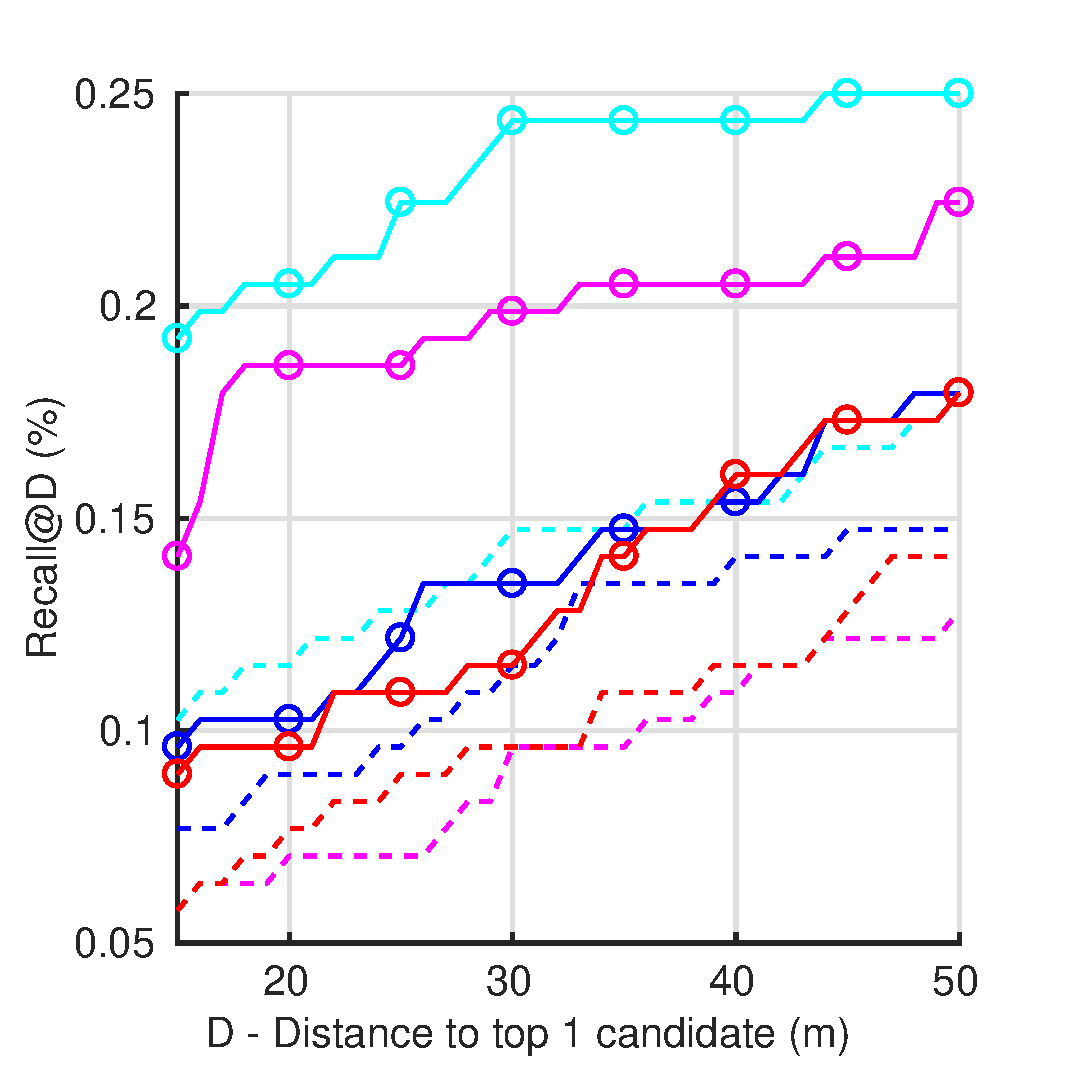
\includegraphics[width=\linewidth]{plot/fig/nightft_distance}	
	\end{minipage}
	\begin{minipage}{0.49\linewidth}
		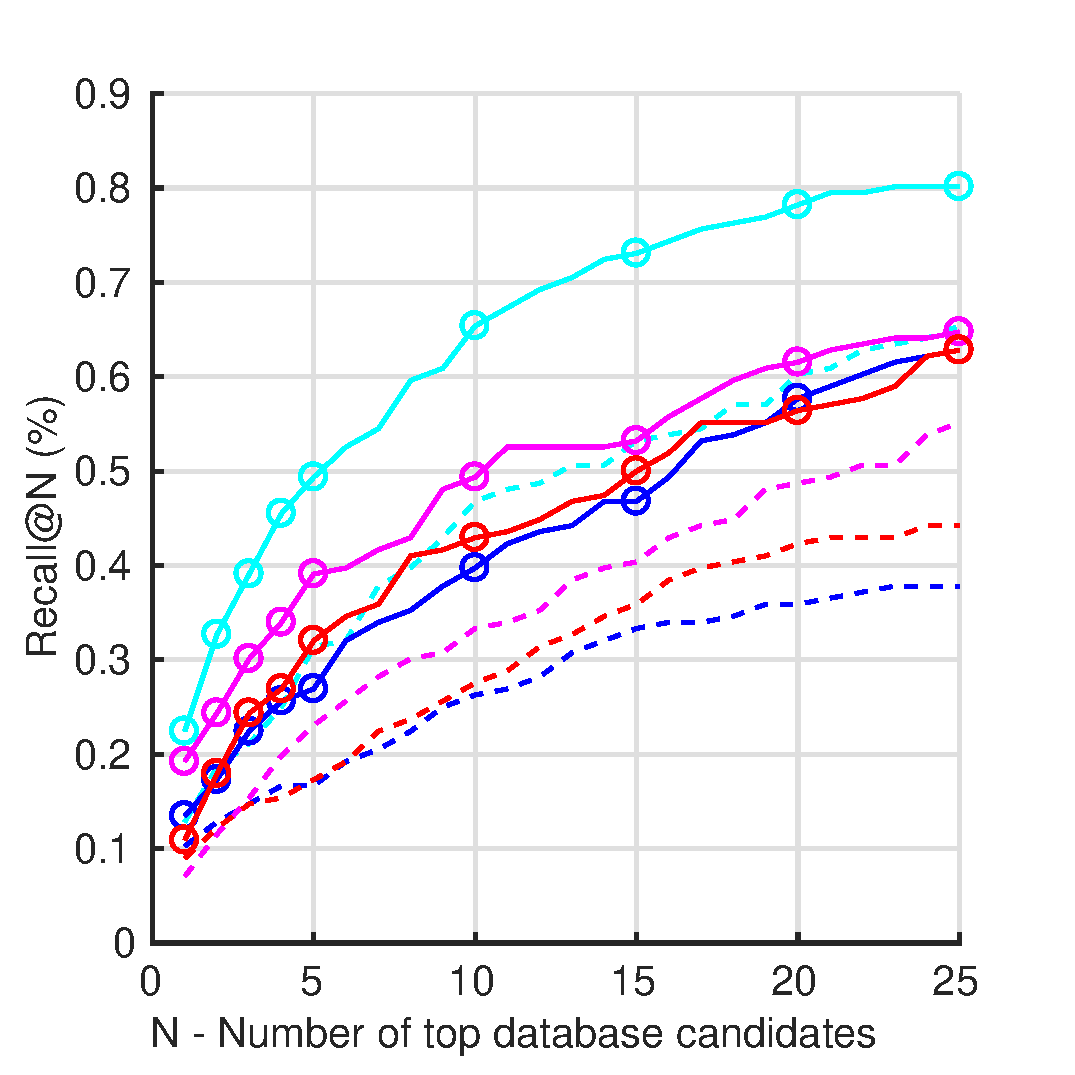
\includegraphics[width=\linewidth]{plot/fig/nightft_recall}	
	\end{minipage}

	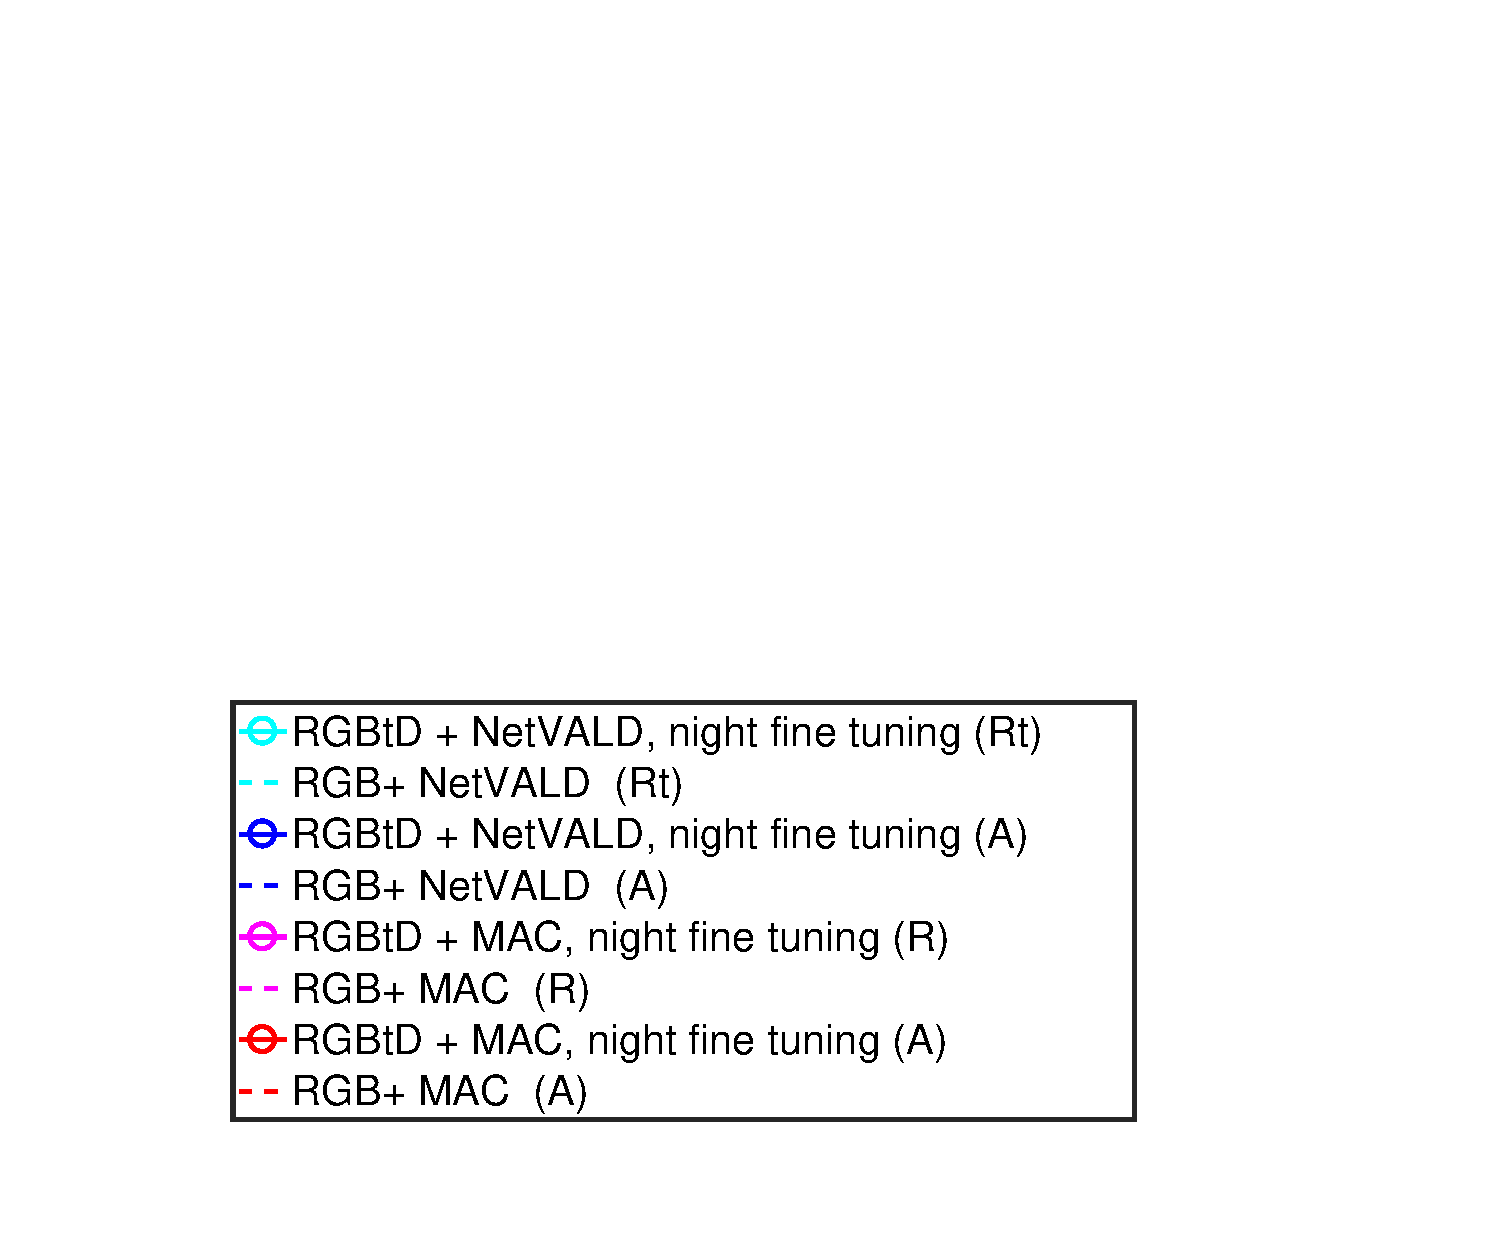
\includegraphics[trim={100 58 165 300},clip,width=0.4\linewidth]{plot/fig/legend_night}
	\caption{\label{fig:ft_night} \textbf{Results on Night/Day query set after fine tuning:} we are able to drastically improve localization performance for the Night/Day challenging scenario by only fine tune the decoder part of our network with weakly annotated data. Best viewed in color.}
\end{figure}
